\chapter{Choix Techniques, Réalisation et Déploiement}

\section{Introduction}
Ce chapitre est consacré à la concrétisation du projet. Nous y justifierons les choix
technologiques adoptés, présenterons la procédure de déploiement sur l'environnement
cible Windows Server 2019, et exposerons les interfaces finales de la plateforme GIA.

\section{Environnement de Déploiement Cible}

\subsection{Justification du Choix : Windows Server 2019}
Conformément au cahier des charges validé par la Direction Informatique de Naftal,
la plateforme a été conçue pour un déploiement sur \textbf{Windows Server 2019}. Ce
choix répond à des exigences stratégiques précises, comme le résume le tableau
comparatif suivant :

% \begin{table}[H]
% \centering
% \begin{tabular}{@{}p{3.5cm}p{4.5cm}p{4.5cm}@{}}
% \toprule
% \textbf{Critère} & \textbf{PC Windows 11 (Dev)} & \textbf{Windows Server 2019 (Prod)} \\ \midrule
% Disponibilité & Dépend de l'utilisateur ; veille fréquente. & Conçu pour tourner \textbf{24h/24, 7j/7}. \\
% Sécurité & Réseau poste de travail, moins contrôlé. & Déploiement on-premise, pare-feu, politiques centralisées. \\
% Usage & Outil individuel. & \textbf{Service mutualisé} pour plusieurs utilisateurs simultanés. \\
% Intégration SI & Isolé du SI d'entreprise. & Nativement intégré au \textbf{réseau intranet Naftal}. \\ \bottomrule
% \end{tabular}
% \caption{Justification du choix de Windows Server 2019 face à un PC standard}
% \label{tab:server}
% \end{table}

\begin{figure}[H]
    \centering
    % On pointe vers le dossier 'figures' et le fichier 'windowsserv19'
    \includegraphics[width=1\textwidth]{figures/windowsserv19.png}
    \caption{Justification du choix de Windows Server 2019 face à un PC standard}
    \label{tab:server}
\end{figure}

\noindent Afin de respecter les exigences de sécurité de Naftal sans perturber le réseau de
production, la plateforme a été simulée et validée sur une \textbf{machine virtuelle
VirtualBox} exécutant Windows Server 2019, prouvant ainsi sa conformité avec les
standards d'infrastructure de l'entreprise.

Avant de détailler la configuration technique, le tableau suivant résume le rôle de chaque
composant dans l'environnement de déploiement GIA.

\begin{table}[H]
\centering
\begin{tabular}{@{}lll@{}}
\toprule
\textbf{Composant} & \textbf{Rôle} & \textbf{Technologie} \\
\midrule
Machine virtuelle & Simule le serveur Naftal & VirtualBox \\
Système d'exploitation & Héberge tous les services & Windows Server 2019 \\
Serveur Web & Reçoit et route les requêtes HTTP & IIS 10 + FastCGI \\
Moteur d'exécution & Interprète la logique métier & PHP 8 (NTS) \\
Base de données & Stocke et protège les données & SQL Server Express 2022 \\
Navigateur client & Interface utilisateur finale & Chrome / Edge (intranet) \\
\bottomrule
\end{tabular}
\caption{Composants de l'environnement de déploiement GIA}
\label{tab:env_deploiement_gia}
\end{table}

\subsection{Configuration du Serveur IIS}
Le service web est assuré par \textbf{IIS (Internet Information Services)}, configuré
avec le module \textbf{FastCGI} pour l'interprétation du PHP. La procédure détaillée ci-dessous
reprend les étapes effectivement suivies sur la machine virtuelle de validation ; elle peut servir
de base à un document d'exploitation pour le centre informatique.

\subsubsection{Phase 1 — Rôle IIS et composants}
Sur Windows Server 2019, ouvrir le \textbf{Gestionnaire de serveur}, ajouter des rôles et
fonctionnalités, choisir \textbf{Serveur Web (IIS)}. Inclure au minimum : services Web de base,
fonctionnalités HTTP communes, et la prise en charge \textbf{CGI} (indispensable pour relier IIS à
PHP via FastCGI). Redémarrer si le système l'exige ; vérifier que la page d'accueil IIS par défaut
répond sur \texttt{localhost}.

\subsubsection{Phase 2 — Installation de PHP}
Télécharger une distribution PHP \textbf{Non Thread Safe (NTS)} compatible avec FastCGI. Extraire
l'arborescence sous \texttt{C:\textbackslash PHP} (ou chemin standardisé par l'entreprise). Copier
\texttt{php.ini-production} vers \texttt{php.ini}. Activer les extensions nécessaires :
\texttt{openssl}, \texttt{curl}, \texttt{mbstring}, \texttt{fileinfo}, et ultérieurement
\texttt{sqlsrv} / \texttt{pdo\_sqlsrv}. Dans le Gestionnaire des services Internet (IIS), au niveau
du serveur, ouvrir \textbf{Mappages de gestionnaire} : ajouter une correspondance de module pour
\texttt{*.php} vers \texttt{FastCgiModule}, avec chemin exécutable \texttt{php-cgi.exe} et arguments
\texttt{-c} pointant vers \texttt{php.ini}. Ajuster \texttt{max\_upload\_filesize} et
\texttt{post\_max\_size} si les pièces jointes incident doivent dépasser la valeur par défaut.

\subsubsection{Phase 3 — SQL Server Express et pilotes}
Installer \textbf{SQL Server Express} (ou édition validée par la DCSI). Activer le protocole TCP/IP
dans le gestionnaire de configuration SQL si les connexions ne sont pas qu'en mémoire partagée.
Créer une base \texttt{GIA\_IncidentDB}, un compte de service ou utiliser l'authentification
Windows selon la politique du site. Installer le \textbf{Microsoft ODBC Driver for SQL Server} et
les DLL PHP \texttt{php\_sqlsrv} / \texttt{php\_pdo\_sqlsrv} correspondant à la version PHP ;
référencer ces extensions dans \texttt{php.ini} et recycler le pool d'applications IIS.

\subsubsection{Phase 4 — Publication du site GIA}
Copier le code applicatif sous \texttt{inetpub\textbackslash wwwroot\textbackslash sonalgaz} (ou
nom normalisé). Créer un \textbf{site IIS} ou une application enfant avec le chemin physique
adéquat ; définir le pool d'applications en \textbf{No Managed Code} pour PHP. Configurer le
document par défaut (\texttt{index.php}). Accorder au compte \texttt{IIS\_IUSRS} (ou identité du
pool) les droits \textbf{Modify}/\textbf{Write} sur le dossier \texttt{uploads/} uniquement
(principe du moindre privilège). Tester un ticket avec pièce jointe pour valider le flux disque.

\subsubsection{Synthèse des quatre phases}
\begin{enumerate}
    \item \textbf{Activation d'IIS} avec CGI.
    \item \textbf{PHP~8.x NTS} + mappage FastCGI + \texttt{php.ini}.
    \item \textbf{SQL Server Express} + pilotes \texttt{sqlsrv} / \texttt{pdo\_sqlsrv}.
    \item \textbf{Déploiement} des fichiers + droits sur \texttt{uploads/}.
\end{enumerate}

\subsection{Contrôles post-installation recommandés}
Après montage de la machine virtuelle ou du serveur cible, les vérifications suivantes réduisent
les incidents d'exploitation :
\begin{enumerate}
    \item Page d'accueil IIS par défaut désactivée ou site GIA défini comme site principal.
    \item Test d'un script \texttt{phpinfo()} retiré en production (fuite d'informations).
    \item Connexion SQL Server depuis PHP (extension \texttt{sqlsrv} / PDO chargée sans erreur
    dans les journaux).
    \item Création d'un compte de chaque rôle (Employé, Technicien, Admin) et parcours complet
    du cycle de vie d'un ticket de bout en bout.
    \item Sauvegarde planifiée de la base \texttt{GIA\_IncidentDB} selon les usages du centre
    informatique.
\end{enumerate}

\section{Outils et Technologies de Développement}

\begin{itemize}
    \item \textbf{Backend — PHP~8 :} Langage côté serveur pour la logique métier.
    La connexion à SQL Server est sécurisée via \textbf{PDO\_SQLSRV} avec requêtes
    paramétrées, prévenant toute injection SQL~\cite{phpdoc}.
    \item \textbf{Frontend — Bootstrap~5 :} Framework CSS open-source pour une
    interface moderne, épurée (style SaaS, effets glassmorphism sur les cartes KPI)
    et \textbf{Responsive Web Design}, s'adaptant aux différentes résolutions d'écran.
    \item \textbf{DataTables :} Librairie JavaScript transformant les tableaux HTML
    en grilles de données interactives avec recherche instantanée, tri multi-colonnes
    et pagination dynamique — sans rechargement de la page.
    \item \textbf{Microsoft SQL Server Express :} SGBD relationnel de Microsoft,
    choisi pour son intégration native avec Windows Server et sa compatibilité avec
    le pilote PHP officiel de Microsoft.
\end{itemize}

\section{Présentation des Interfaces de l'Application}

\subsection{La Page de Connexion}
La première interface de la plateforme est un formulaire de connexion sécurisé.
Après soumission, PHP vérifie les identifiants, compare le mot de passe au hash
stocké en base (\texttt{password\_verify}), et initialise une session PHP
(\texttt{\$\_SESSION}) stockant l'identifiant et le rôle de l'utilisateur.
\begin{figure}[H]
    \centering
    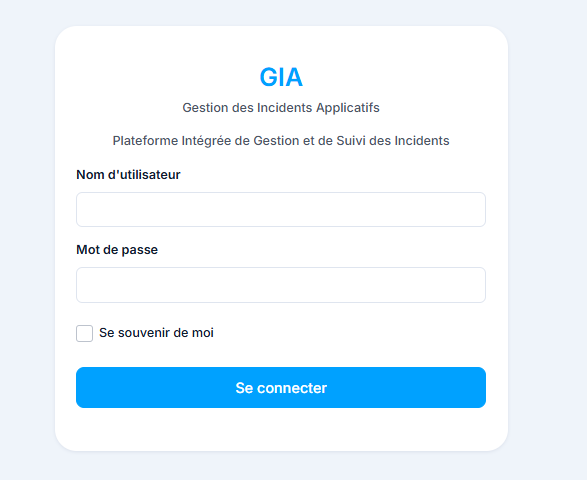
\includegraphics[width=0.92\textwidth]{figures/capture_login.png}
    \caption{Page de connexion de la plateforme GIA}
\end{figure}

\subsection{Le Tableau de Bord de l'Administrateur}
L'interface de l'Administrateur offre une \textbf{supervision globale et en temps
réel}. La partie haute affiche des \textbf{cartes KPI} dynamiques générées par des
requêtes SQL de comptage (\texttt{COUNT} avec \texttt{GROUP BY}) présentant :
le nombre total de tickets, les tickets ouverts non assignés, les tickets résolus cette
semaine, et le nombre de techniciens actifs.
\begin{figure}[H]
    \centering
    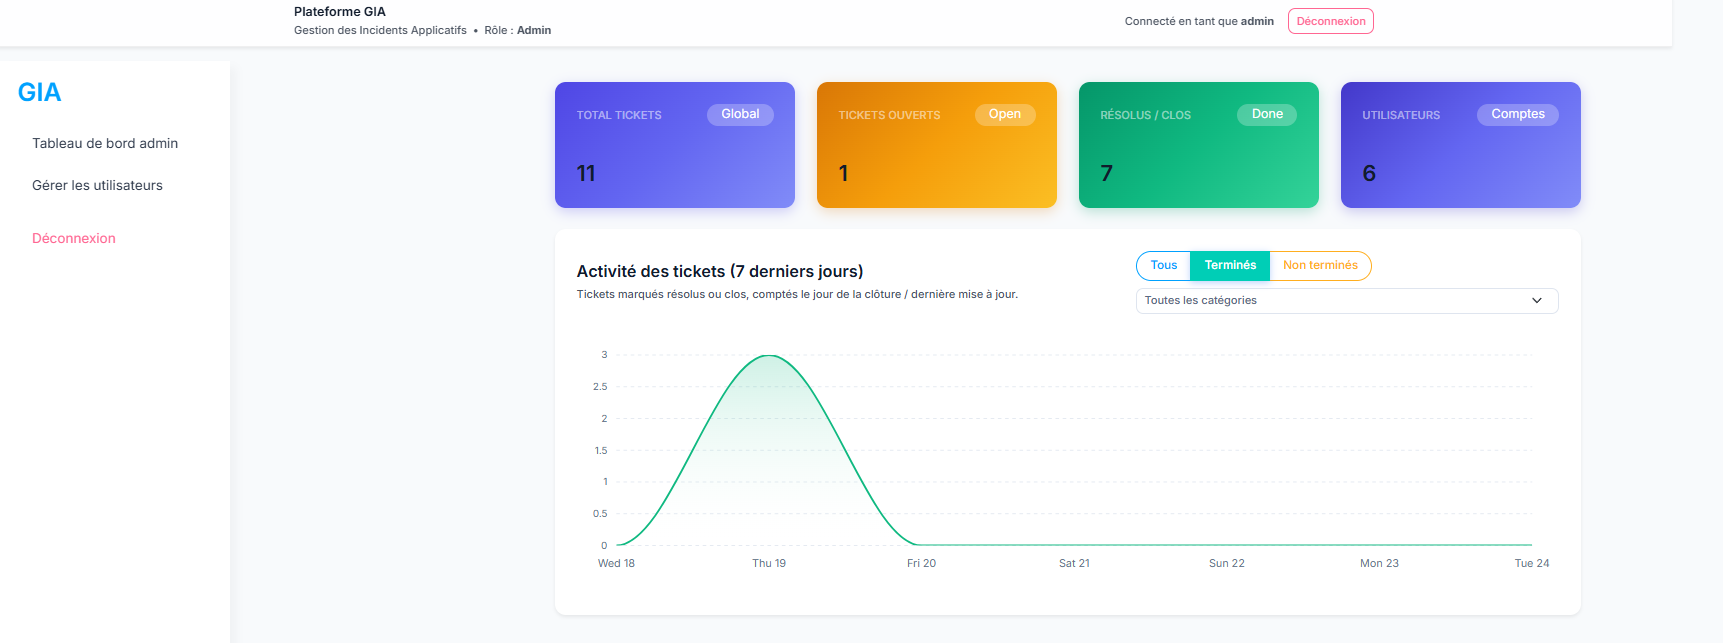
\includegraphics[width=0.92\textwidth]{figures/capture_admin_dashboard.png}
    \caption{Tableau de bord de l'Administrateur — KPIs et suivi global}
\end{figure}

\subsection{La Liste des Tickets (DataTables)}
La page de suivi centralise l'ensemble des tickets dans une grille \textbf{DataTables}
interactive. L'utilisateur peut filtrer instantanément, trier par colonnes (statut,
priorité, date) et naviguer par pagination, ce qui améliore la traçabilité et la
rapidité de consultation sans rechargement complet de la page.
\begin{figure}[H]
    \centering
    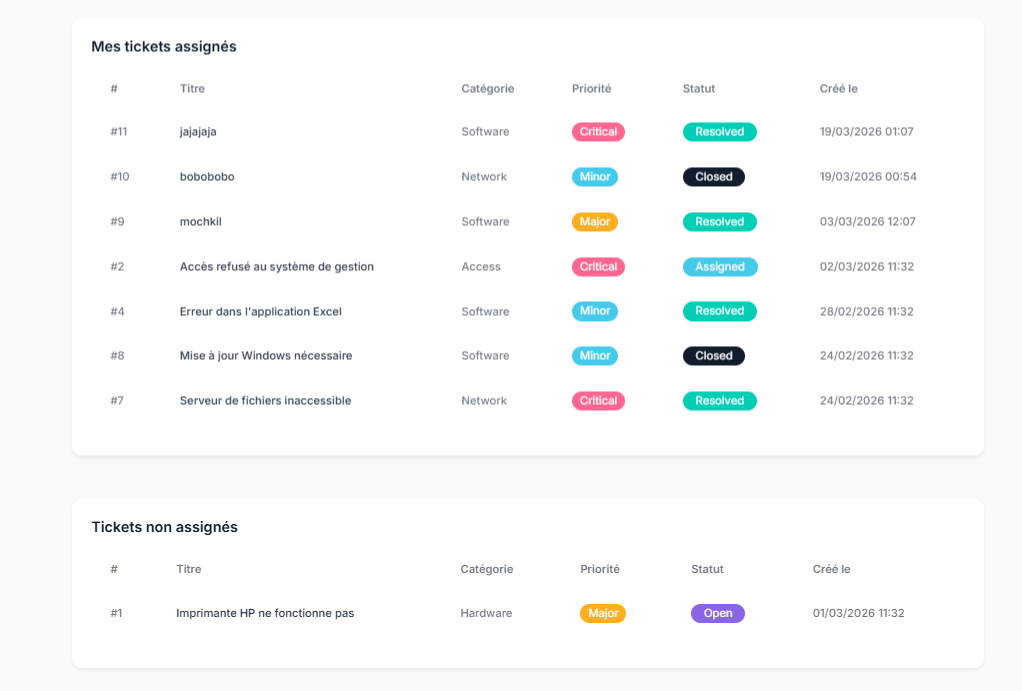
\includegraphics[width=0.92\textwidth]{figures/capture_liste_tickets.png}
    \caption{Screenshot de la liste des tickets (DataTables)}
\end{figure}

\subsection{La Vue Technicien : Traitement d'un Ticket}
Lorsqu'un Technicien consulte un ticket, l'interface est divisée en deux zones
ergonomiques. À gauche : les détails complets du problème et la \textbf{timeline
chronologique} des actions passées (extraite de \texttt{incident\_logs}), visualisant
l'historique complet de l'incident. À droite : le panneau d'action pour changer le
statut, rédiger un rapport de diagnostic ou ajouter un commentaire.
\begin{figure}[H]
    \centering
    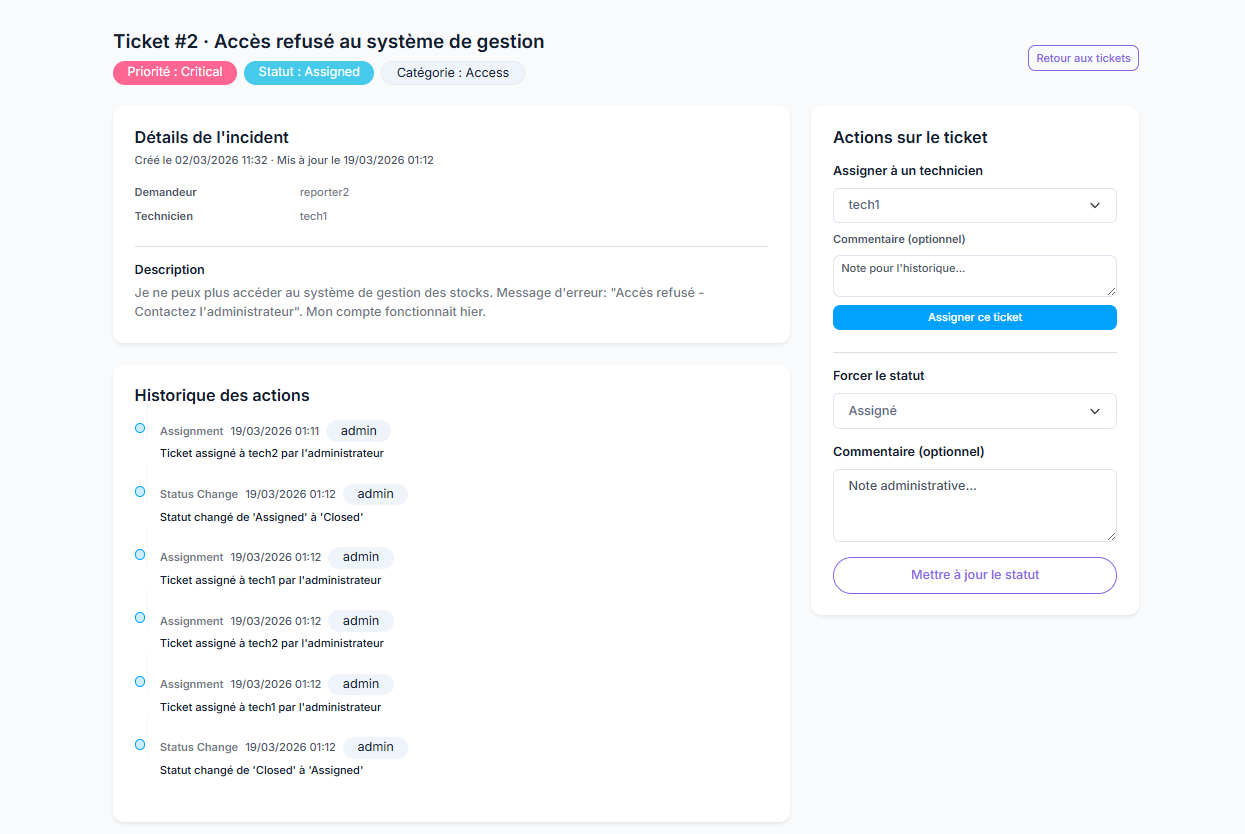
\includegraphics[width=0.92\textwidth]{figures/capture_vue_ticket.png}
    \caption{Interface de traitement d'un ticket — Timeline et panneau d'action}
\end{figure}

\subsection{Le Formulaire de Création de Ticket (Demandeur)}
L'Employé accède à un formulaire structuré et intuitif pour déclarer un incident.
Il renseigne le titre, sélectionne la catégorie applicative et le niveau de priorité
(Critique, Majeur, Mineur) dans des listes déroulantes Bootstrap, saisit une
description détaillée et peut attacher une capture d'écran. À la soumission, le
système crée la ligne dans \texttt{incidents} avec le statut \texttt{Ouvert} et
enregistre l'événement \texttt{Creation} dans \texttt{incident\_logs}.
\begin{figure}[H]
    \centering
    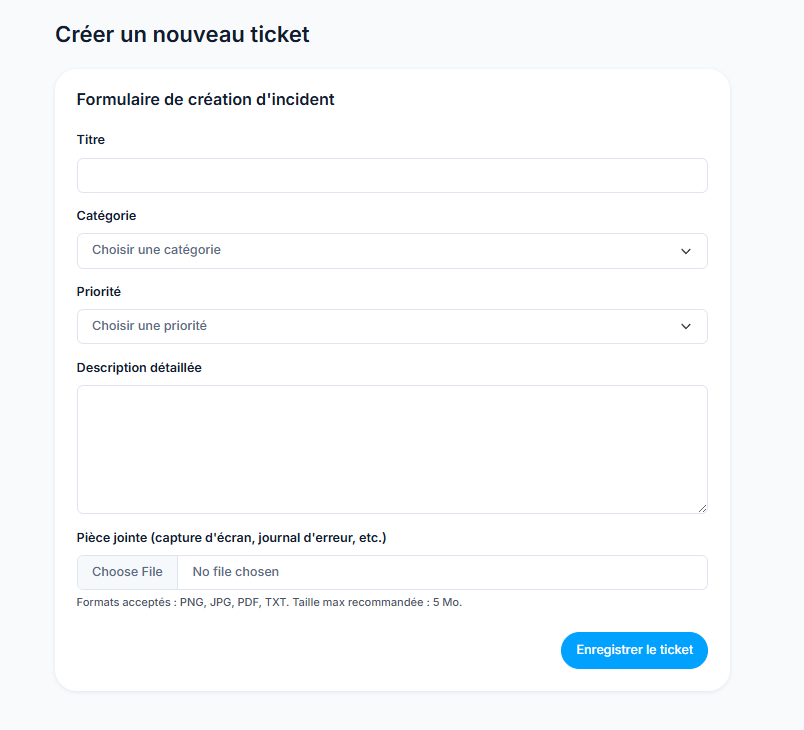
\includegraphics[width=0.92\textwidth]{figures/capture_create_ticket.png}
    \caption{Formulaire de création de ticket côté Demandeur}
\end{figure}

\section{Conclusion}
La phase de réalisation a permis de transformer le modèle conceptuel en une
solution logicielle fonctionnelle, robuste et parfaitement adaptée aux contraintes
d'infrastructure de Naftal. Déployée sur Windows Server 2019 avec IIS et SQL Server,
la plateforme GIA répond à l'ensemble des exigences du cahier des charges initial.
